\documentclass[11pt]{article}

% ------
% LAYOUT
% ------
\textwidth 165mm %
\textheight 230mm %
\oddsidemargin 0mm %
\evensidemargin 0mm %
\topmargin -15mm %
\parindent= 10mm

\usepackage[dvips]{graphicx}
\usepackage{multirow,multicol}
\usepackage[table]{xcolor}

\usepackage{amssymb}
\usepackage{amsfonts}
\usepackage{amsthm}
\usepackage{amsmath}

\usepackage{subfigure}
\usepackage{minted}

\graphicspath{{./pix/}} % put all your figures here.

\begin{document}
\begin{center}
\Large{\textbf{ECE 595: Homework 3}}

Yi Qiao, Class ID 187

(Spring 2019)
\end{center}

\section*{Exercise 1}
\subsection*{(a)}
\subsubsection*{(i)}
\noindent \textbf{To Prove:}$$\pmb{x}^T\pmb{Ax}=tr\left[\pmb{Axx}^T\right]$$

\begin{equation}
\begin{split}
\pmb{x}^T\pmb{Ax} &=\begin{bmatrix}
x_0 & x_1 & ... & x_{n-1}
\end{bmatrix}\begin{bmatrix}
a_{0,0} & a_{0,1} & ... & a_{0,n-1}\\
\vdots  &	\vdots & 	&	\vdots \\
a_{n-1,0}&	a_{n-1,1} & ... & a_{n-1, n-1}\\
\end{bmatrix}\begin{bmatrix}
x_0\\
x_1\\
\vdots\\
x_{n-1}\\
\end{bmatrix}\\
&=\sum_{j=0}^{n-1}\sum_{i=0}^{n-1}x_ia_{i,j}x_j\\
&=\sum_{i=0}^{n-1}\left(\sum_{j=0}^{n-1}a_{i,j}x_j\right)x_i\\
\end{split}
\end{equation}
\begin{equation}
\begin{split}
tr\left[\pmb{Axx}^T\right]&=tr\left[\begin{bmatrix}
-\ a_0\ -\pmb{x} \\
-\ a_1\ -\pmb{x} \\
\vdots \\
-\ a_{n-1}\ -\pmb{x}
\end{bmatrix}\pmb{x}^T\right]\\
&=tr\left[\begin{bmatrix}
-\ a_0\ -\pmb{x}x_{0} & -\ a_0\ -\pmb{x}x_1 & ... & -\ a_0\ -\pmb{x}x_{n-1} \\
-\ a_1\ -\pmb{x}x_{0} & -\ a_1\ -\pmb{x}x_1 & ... & -\ a_1\ -\pmb{x}x_{n-1}\\
\vdots & \vdots & ... & \vdots \\
-\ a_{n-1}\ -\pmb{x}x_{0} & -\ a_{n-1}\ -\pmb{x}x_{0} & ... & -\ a_{n-1}\ -\pmb{x}x_{0}
\end{bmatrix}\right]\\
&=\sum_{i=0}^{n-1}-\ a_i\ -\pmb{x}x_i\\
&=\sum_{i=0}^{n-1}\left(\sum_{j=0}^{n-1}a_{i,j}x_j\right)x_i
\end{split}
\end{equation}\\
Thus, the above two are equivalent.
\pagebreak
\subsubsection*{(ii)}

since the likelihood function is, $$p(\pmb{x}|\pmb{\Sigma})=\frac{1}{(2\pi)^{d/2}|\pmb{\Sigma}|^{1/2}}exp\left\{-\frac{1}{2}(\pmb{x}-\pmb{\mu})^T\pmb{\Sigma}^{-1}(\pmb{x}-\pmb{\mu})\right\}$$

\begin{equation}
\begin{split}
p(\pmb{x}_1,...,\pmb{x}_N|\pmb{\Sigma})&=\prod_{i=1}^{N}\frac{1}{(2\pi)^{d/2}|\pmb{\Sigma}|^{1/2}}exp\left\{-\frac{1}{2}(\pmb{x}_i-\pmb{\mu})^T\pmb{\Sigma}^{-1}(\pmb{x}_i-\pmb{\mu})\right\}\\
&=\frac{1}{(2\pi)^{Nd/2}}|\pmb{\Sigma}^{-1}|^{N/2}exp\left\{-\frac{1}{2}\sum_{i=1}^{N}(\pmb{x}_i-\pmb{\mu})^T\pmb{\Sigma}^{-1}(\pmb{x}_i-\pmb{\mu})\right\}\\
\end{split}
\end{equation}\\

Using the property we found above, we get,

\begin{equation}
\begin{split}
p(\pmb{x}_1,...,\pmb{x}_N|\pmb{\Sigma})&=\frac{1}{(2\pi)^{Nd/2}}|\pmb{\Sigma}^{-1}|^{N/2}exp\left\{-\frac{1}{2}\sum_{i=1}^{N}tr\left[\pmb{\Sigma}^{-1}(\pmb{x}_i-\pmb{\mu})(\pmb{x}_i-\pmb{\mu})^T\right]\right\}\\
&=\frac{1}{(2\pi)^{Nd/2}}|\pmb{\Sigma}^{-1}|^{N/2}exp\left\{-\frac{1}{2}tr\left[\sum_{i=1}^{N}\pmb{\Sigma}^{-1}(\pmb{x}_i-\pmb{\mu})(\pmb{x}_i-\pmb{\mu})^T\right]\right\}\\
&=\frac{1}{(2\pi)^{Nd/2}}|\pmb{\Sigma}^{-1}|^{N/2}exp\left\{-\frac{1}{2}tr\left[\pmb{\Sigma}^{-1}\sum_{i=1}^{N}(\pmb{x}_i-\pmb{\mu})(\pmb{x}_i-\pmb{\mu})^T\right]\right\}
\end{split}
\end{equation}

\subsubsection*{(iii)}
since 
$$\hat{\pmb{\Sigma}}_{MLE} = \frac{1}{N}\sum_{n=1}^{N}(\pmb{x}_n-\hat{\pmb{\mu}})(\pmb{x}_n-\hat{\pmb{\mu}})^T$$
we can rewrite the equation above as\\
\begin{equation}
\begin{split}
p(\pmb{x}_1,...,\pmb{x}_N|\pmb{\Sigma})&=\frac{1}{(2\pi)^{Nd/2}}|\pmb{A}\hat{\pmb{\Sigma}}_{MLE}^{-1}|^{N/2}exp\left\{-\frac{1}{2}tr\left[\pmb{\Sigma}^{-1}N\hat{\pmb{\Sigma}}_{MLE}\right]\right\}\\
&=\frac{1}{(2\pi)^{Nd/2}|\hat{\pmb{\Sigma}}_{MLE}|^{N/2}}|\pmb{A}|^{N/2}exp\left\{-\frac{N}{2}tr\left[A\right]\right\}\\
\end{split}
\end{equation}
since $\pmb{A}$ is diagonalizable, $|\pmb{A}| = \prod_{i=1}^{d}\lambda_i$, plug it in, we get

\begin{equation}
\begin{split}
p(\pmb{x}_1,...,\pmb{x}_N|\pmb{\Sigma})&=\frac{1}{(2\pi)^{Nd/2}|\hat{\pmb{\Sigma}}_{MLE}|^{N/2}}(\prod_{i=1}^{d}\lambda_i)^{N/2}exp\left\{-\frac{N}{2}\sum_{i=1}^{d}\lambda_i\right\}\\
\end{split}
\end{equation}

\pagebreak
\subsubsection*{(iv)}
To maximize the likelihood function $$\underset{\lambda_1...\lambda_d}{argmax}\ p(x_1,...,x_N|\pmb{\Sigma})$$
we have,
\begin{equation}
\begin{split}
\pmb{\lambda}&=\underset{\lambda_1...\lambda_d}{argmax}\  \frac{1}{(2\pi)^{Nd/2}|\hat{\pmb{\Sigma}}_{MLE}|^{N/2}}(\prod_{i=1}^{d}\lambda_i)^{N/2}exp\left\{-\frac{N}{2}\sum_{i=1}^{d}\lambda_i\right\}\\
&=\underset{\lambda_1...\lambda_d}{argmax}\ (\prod_{i=1}^{d}\lambda_i)^{N/2}exp\left\{-\frac{N}{2}\sum_{i=1}^{d}\lambda_i\right\}\\
&=\underset{\lambda_1...\lambda_d}{argmin}\ -log(\prod_{i=1}^{d}\lambda_i)+\sum_{i=1}^{d}\lambda_i\\
&=\underset{\lambda_1...\lambda_d}{argmin}\ -\sum_{i=1}^{d}log(\lambda_i)+\sum_{i=1}^{d}\lambda_i\\
&=\underset{\lambda_1...\lambda_d}{argmin}\ \sum_{i=1}^{d}\lambda_i-log(\lambda_i)\\
\end{split}
\end{equation}

Take derivative, setting to zero:
$$\nabla\pmb{\lambda}= \begin{bmatrix}
1-\frac{1}{\lambda_1}\\
1-\frac{1}{\lambda_2}\\
\vdots\\
1-\frac{1}{\lambda_d}\\
\end{bmatrix} = \pmb{0}$$

Obviously $\lambda_i=1$ for all $i$.
\subsection*{(b)}
By maximizing the likelihood function:
$$\hat{\pmb{\Sigma}} = \underset{\pmb{\Sigma}}{argmax}\ p(\pmb{x}_1,...,\pmb{x}_N|\pmb{\Sigma})$$
\begin{equation}
\begin{split}
\hat{\pmb{\Sigma}}&=\underset{\pmb{\Sigma}}{argmax}\ \frac{1}{(2\pi)^{Nd/2}|\pmb{\Sigma}|^{N/2}}exp\left\{-\frac{1}{2}\sum_{i=1}^{N}(\pmb{x}_i-\pmb{\mu})^T\pmb{\Sigma}^{-1}(\pmb{x}_i-\pmb{\mu})\right\}\\
&=\underset{\pmb{\Sigma}}{argmax}\  \frac{|\pmb{\Sigma}^{-1}|^{N/2}}{(2\pi)^{Nd/2}}exp\left\{-\frac{1}{2}tr\left[\pmb{\Sigma}^{-1}\sum_{i=1}^{N}(\pmb{x}_i-\pmb{\mu})(\pmb{x}_i-\pmb{\mu})^T\right]\right\}\\
&=\underset{\pmb{\Sigma}}{argmin}\ -\frac{N}{2}log(|\pmb{\Sigma}^{-1}|)+\frac{Nd}{2}log(2\pi)+\frac{1}{2}tr\left[\pmb{\Sigma}^{-1}\sum_{i=0}^{N}(\pmb{x}_i-\pmb{\mu})(\pmb{x}_i-\pmb{\mu})^T\right]\\
&=\underset{\pmb{\Sigma}}{argmin}\ -Nlog(|\pmb{\Sigma}^{-1}|)+tr\left[\pmb{\Sigma}^{-1}\sum_{i=0}^{N}(\pmb{x}_i-\pmb{\mu})(\pmb{x}_i-\pmb{\mu})^T\right]
\end{split}
\end{equation}
\pagebreak

\noindent Set $\pmb{P} = \pmb{\Sigma}^{-1}$\\
\begin{equation}
\begin{split}
\hat{\pmb{P}} = \underset{\pmb{P}}{argmin}\ -Nlog(|\pmb{P}|)+tr\left[\pmb{P}\sum_{i=0}^{N}(\pmb{x}_i-\pmb{\mu})(\pmb{x}_i-\pmb{\mu})^T\right]
\end{split}
\end{equation}
Take derivative, setting to zero:
\begin{equation}
\begin{split}
-\frac{N}{|\pmb{P}|}|\pmb{P}|\pmb{P}^{-1}&+\sum_{i=0}^{N}(\pmb{x}_i-\pmb{\mu})(\pmb{x}_i-\pmb{\mu})^T = 0\\
N\pmb{P}^{-1}&=\sum_{i=0}^{N}(\pmb{x}_i-\pmb{\mu})(\pmb{x}_i-\pmb{\mu})^T\\
\pmb{P}^{-1}&=\frac{1}{N}\sum_{i=0}^{N}(\pmb{x}_i-\pmb{\mu})(\pmb{x}_i-\pmb{\mu})^T\\
\end{split}
\end{equation}
thus,

$$\hat{\pmb{\Sigma}}_{MLE}=\frac{1}{N}\sum_{i=0}^{N}(\pmb{x}_i-\pmb{\mu})(\pmb{x}_i-\pmb{\mu})^T$$

\section*{Exercise 2}
\subsection*{(a)}
\noindent Refer to code in the back
\subsection*{(b)}
\subsubsection*{(i),(ii) \& (iii)}
\begin{figure}[h]
	\centering
	\subfigure[overlapping pathces]{
		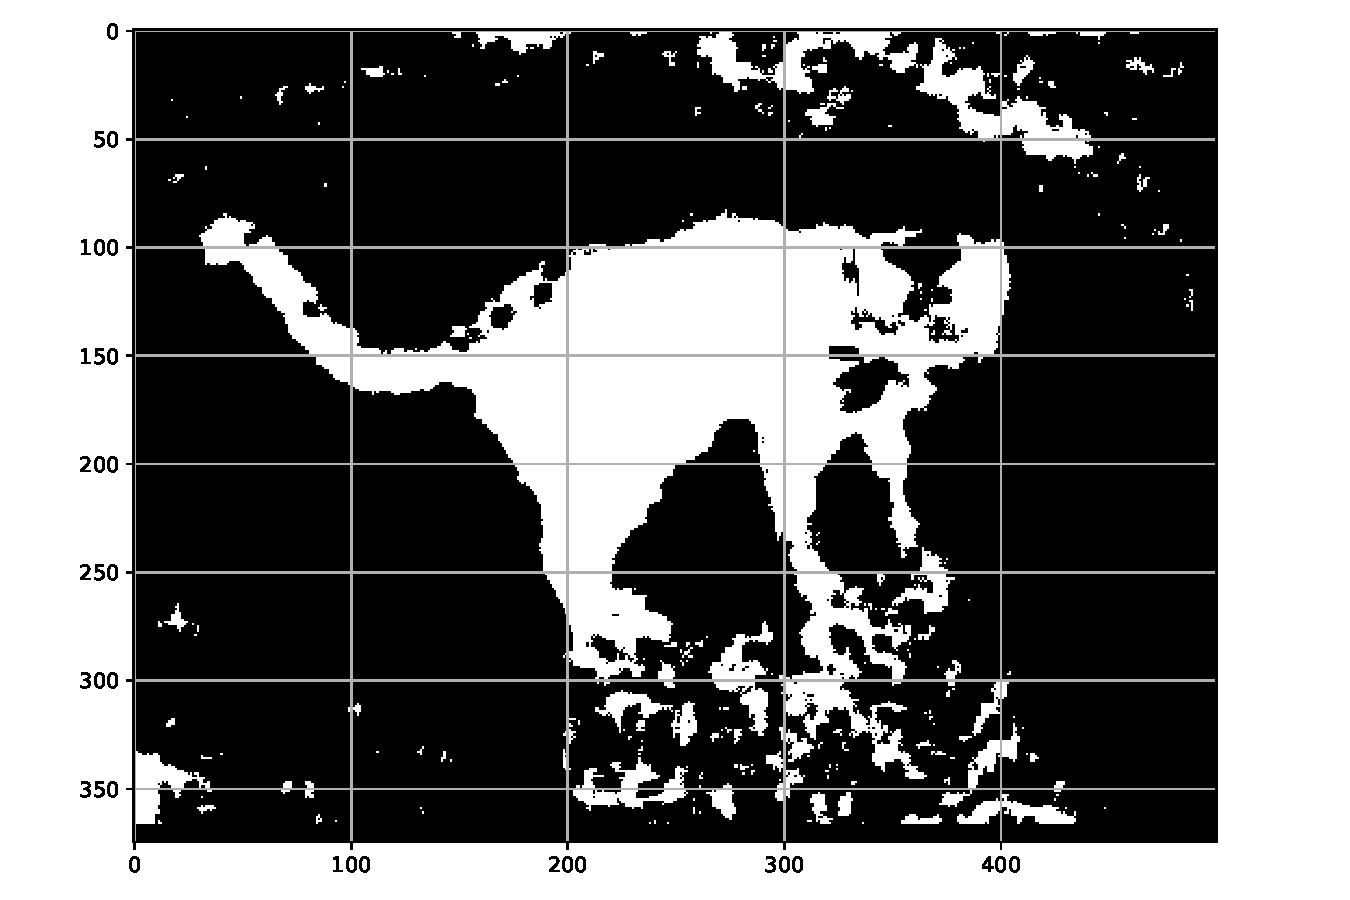
\includegraphics[width=0.47\linewidth]{overlapping_output}
	}
	\subfigure[non-overlapping pathces]{
		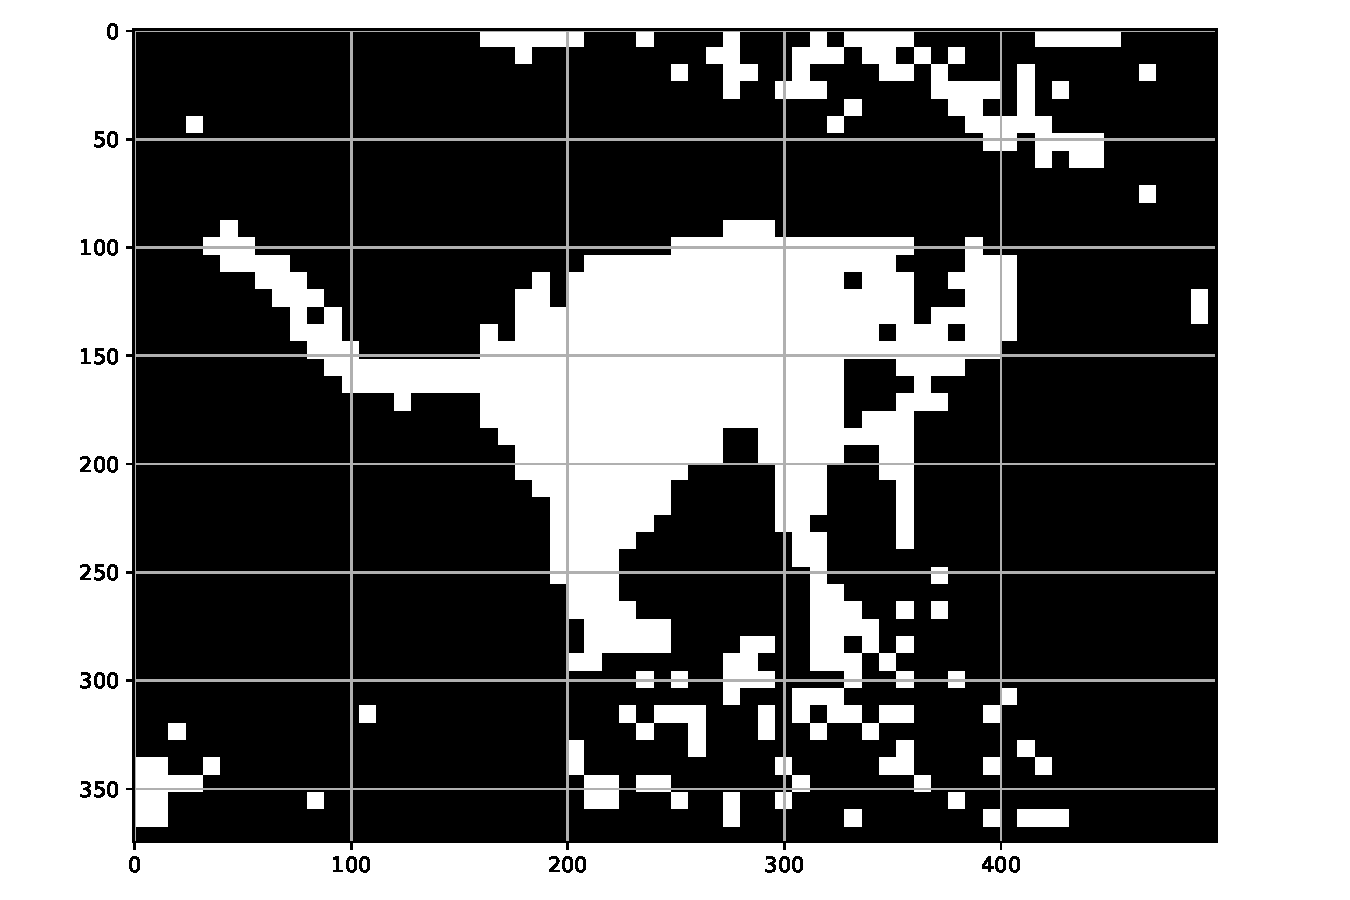
\includegraphics[width=0.47\linewidth]{non_overlapping_output}
	}
	\caption{MAP classifier}
\end{figure}

\subsubsection*{(iv)}
	$$MAE_{overlapping} = 0.00945$$
	$$MAE_{non-overlapping} = 0.00985$$
	
\subsubsection*{(v)}
\begin{figure}[h]
	\centering
	\subfigure[original]{
		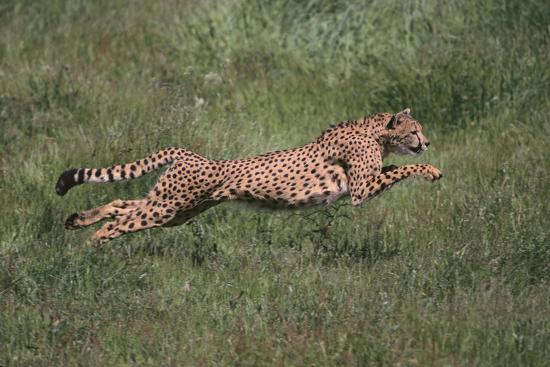
\includegraphics[width=0.47\linewidth]{../data/test}
	}
	\subfigure[classified]{
		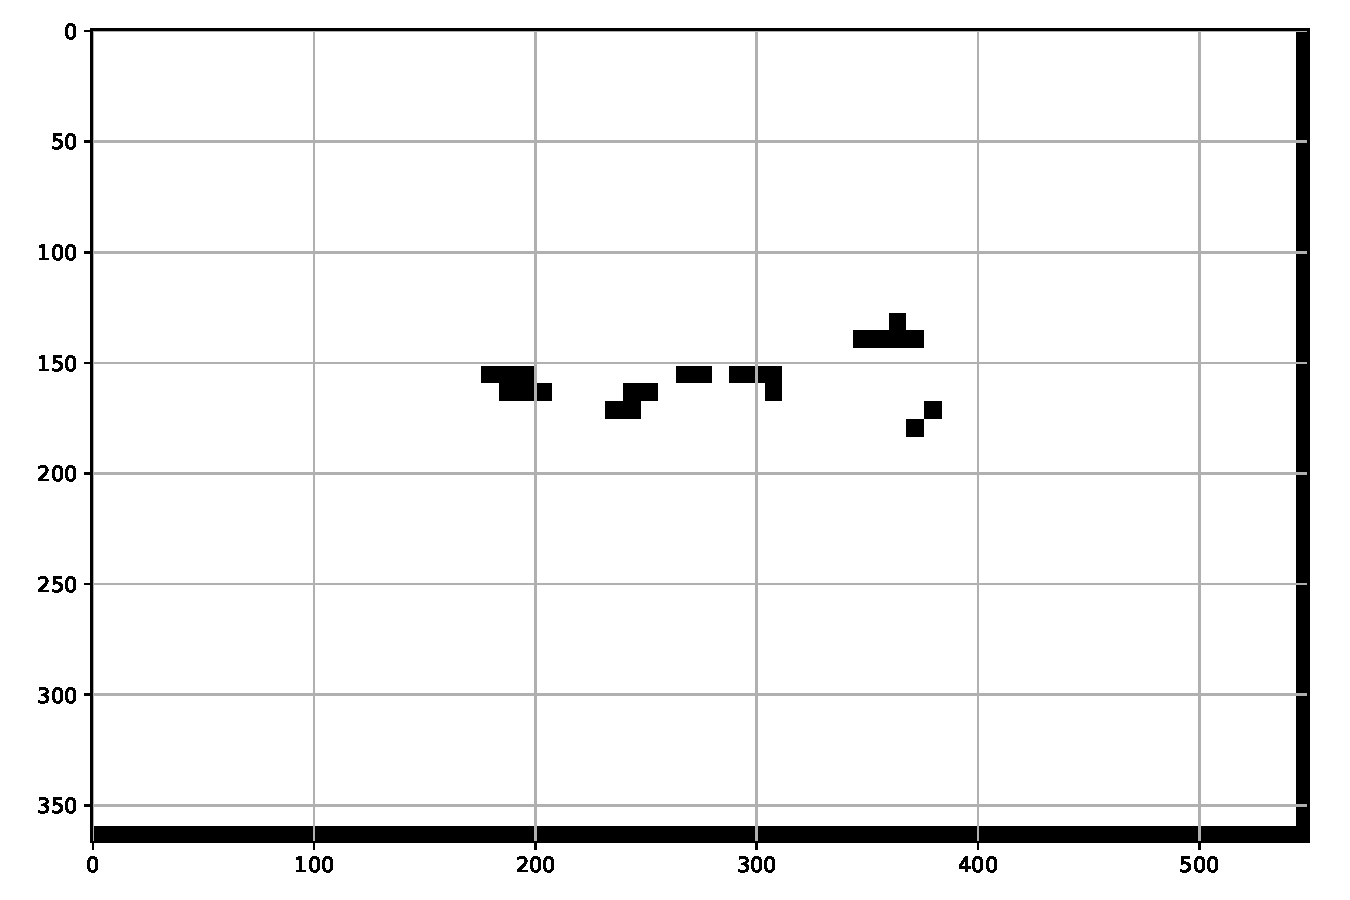
\includegraphics[width=0.47\linewidth]{non_overlapping_test}
	}
	\caption{MAP classifier}
\end{figure}

\noindent Obviously, this classifier is not working at all when using with other pictures.\\
Why?\\
The training data is too small. (Probably the training data comes from the testing picture, thus performing well on it)\\
The prior is not "good" by simply using the ratio of data points. Its a estimation that does not make sense generically.

\pagebreak
\section*{Exercise 3}
\subsection*{(a)}
For a Gaussian classifier with same covariance matrix across the board, the decision boundary is,
$$g(\pmb{x}) = \pmb{\beta}^T(\pmb{x}-\beta_0)=0$$
with,
$$\pmb{\beta} = \pmb{\Sigma}^{-1}(\pmb{\mu}_i-\pmb{\mu}_j)$$
$$\beta_0=\frac{\pmb{\mu}_i+\pmb{\mu}_j}{2}-\frac{log\frac{\pi_i}{\pi_j}}{(\pmb{\mu}_i-\pmb{\mu}_j)^T\pmb{\Sigma}^{-1}(\pmb{\mu}_i-\pmb{\mu}_j)}(\pmb{\mu}_i-\pmb{\mu}_j)$$

\subsection*{(b)}
\subsubsection*{(i)}
\noindent \textbf{To Prove:}
$$\pmb{A}^T\pmb{A}=\begin{bmatrix}
(N-2)\hat{\pmb{\Sigma}}+N_1\hat{\pmb{\mu}}_1\hat{\pmb{\mu}}_1^T+N_2\hat{\pmb{\mu}}_2\hat{\pmb{\mu}}_2^T & N_1\hat{\pmb{\mu}_1}+N_2\hat{\pmb{\mu}_2}\\
N_1\hat{\pmb{\mu}_1}^T+N_2\hat{\pmb{\mu}_2}^T & N
\end{bmatrix}$$

\begin{equation}
\begin{split}
\pmb{A}^T\pmb{A}&=\begin{bmatrix}
|&&|&|&&|\\
\pmb{x}^{(1)}_1&...&\pmb{x}^{(1)}_{N1}&\pmb{x}^{(2)}_1&...&\pmb{x}^{(2)}_{N2}\\
|&&|&|&&|\\
1&...&1&1&...&1\\
\end{bmatrix}\begin{bmatrix}
-\pmb{x}^{(1)T}_1-& 1\\
\vdots&\vdots\\
-\pmb{x}^{(1)T}_{N1}-& 1\\
-\pmb{x}^{(2)T}_1-& 1\\
\vdots&\vdots\\
-\pmb{x}^{(2)T}_{N2}-& 1\\
\end{bmatrix}\\
&=\begin{bmatrix}
\begin{bmatrix}
|&&|&|&&|\\
\pmb{x}^{(1)}_1&...&\pmb{x}^{(1)}_{N1}&\pmb{x}^{(2)}_1&...&\pmb{x}^{(2)}_{N2}\\
|&&|&|&&|\\
\end{bmatrix}\begin{bmatrix}
-\pmb{x}^{(1)T}_1-\\
\vdots\\
-\pmb{x}^{(1)T}_{N1}-\\
-\pmb{y}^{(2)T}_1-\\
\vdots\\
-\pmb{y}^{(2)T}_{N2}-\\
\end{bmatrix}
&\begin{bmatrix}
|&&|&|&&|\\
\pmb{x}^{(1)}_1&...&\pmb{x}^{(1)}_{N1}&\pmb{x}^{(2)}_1&...&\pmb{x}^{(2)}_{N2}\\
|&&|&|&&|\\
\end{bmatrix}\begin{bmatrix}
1\\
\vdots\\
1\\
1\\
\vdots\\
1\\
\end{bmatrix}\\
\begin{bmatrix}
1&...&1&1&...&1
\end{bmatrix}\begin{bmatrix}
-\pmb{x}^{(1)T}_1-\\
\vdots\\
-\pmb{x}^{(1)T}_{N1}-\\
-\pmb{x}^{(2)T}_1-\\
\vdots\\
-\pmb{x}^{(2)T}_{N2}-\\
\end{bmatrix}&
\begin{bmatrix}
1&...&1&1&...&1
\end{bmatrix}\begin{bmatrix}
1\\
\vdots\\
1\\
1\\
\vdots\\
1\\
\end{bmatrix}\\
\end{bmatrix}\\
&=\begin{bmatrix}
\sum_{i=1}^{N1}\pmb{x}^{(1)}_i\pmb{x}^{(1)T}_i+\sum_{i=1}^{N2}\pmb{x}^{(2)}_i\pmb{x}^{(2)T}_i&\sum_{i=1}^{N1}\pmb{x}^{(1)}_i + \sum_{i=1}^{N2}\pmb{x}^{(2)}_i\\
\sum_{i=1}^{N1}\pmb{x}^{(1)T}_i + \sum_{i=1}^{N2}\pmb{x}^{(2)T}_i&N_1+N_2\\
\end{bmatrix}\\
&=\begin{bmatrix}
(N-2)\hat{\pmb{\Sigma}}+\sum_{j=1}^{2}\sum_{i=1}^{N_j}\hat{\pmb{\mu}}_j\pmb{x}^{(j)T}_i+\pmb{x}^{(j)}\hat{\pmb{\mu}}^T_j-\hat{\pmb{\mu}}_j\hat{\pmb{\mu}}^T_j&N_1\pmb{\mu}_1+N_2\pmb{\mu}_2\\
N_1\hat{\pmb{\mu}}^T_1+N_2\hat{\pmb{\mu}}^T_2&N\\
\end{bmatrix}
\end{split}
\end{equation}

The top left term,
$$(N-2)\hat{\pmb{\Sigma}}+\sum_{j=1}^{2}\sum_{i=1}^{N_j}\hat{\pmb{\mu}}_j\pmb{x}^{(j)T}_i+\pmb{x}^{(j)}\hat{\pmb{\mu}}^T_j-\hat{\pmb{\mu}}_j\hat{\pmb{\mu}}^T_j$$
can be simplified as follow,
\begin{equation}
\begin{split}
(N-2)\hat{\pmb{\Sigma}}+&\sum_{j=1}^{2}\sum_{i=1}^{N_j}\hat{\pmb{\mu}}_j\pmb{x}^{(j)T}_i+\pmb{x}^{(j)}_i\hat{\pmb{\mu}}^T_j-\hat{\pmb{\mu}}_j\hat{\pmb{\mu}}^T_j\\
&=(N-2)\hat{\pmb{\Sigma}}+\sum_{j=1}^{2}\sum_{i=1}^{N_j}\left(\frac{1}{N_j}\sum_{k=1}^{N_j}\pmb{x}^{(j)}_k\right)\pmb{x}^{(j)T}_i+\pmb{x}^{(j)}_i\left(\frac{1}{N_j}\sum_{k=1}^{N_j}\pmb{x}^{(j)T}_k\right)-\hat{\pmb{\mu}}_j\hat{\pmb{\mu}}^T_j\\
&=(N-2)\hat{\pmb{\Sigma}}+\sum_{j=1}^{2}\left(\frac{1}{N_j}\sum_{i=1}^{N_j}\sum_{k=1}^{N_j}\pmb{x}^{(j)}_k\pmb{x}^{(j)T}_i\right)+\left(\frac{1}{N_j}\sum_{i=1}^{N_j}\sum_{k=1}^{N_j}\pmb{x}^{(j)}_i\pmb{x}^{(j)T}_k\right)-N_j\hat{\pmb{\mu}}_j\hat{\pmb{\mu}}^T_j\\
&=(N-2)\hat{\pmb{\Sigma}}+\sum_{j=1}^{2}N_j\hat{\pmb{\mu}}_j\hat{\pmb{\mu}}^T_j+N_j\hat{\pmb{\mu}}_j\hat{\pmb{\mu}}^T_j-N_j\hat{\pmb{\mu}}_j\hat{\pmb{\mu}}^T_j\\
&=(N-2)\hat{\pmb{\Sigma}}+N_1\hat{\pmb{\mu}}_1\hat{\pmb{\mu}}^T_1+N_2\hat{\pmb{\mu}}_2\hat{\pmb{\mu}}^T_2
\end{split}
\end{equation}
Substitute back, we get,
$$\pmb{A}^T\pmb{A}=\begin{bmatrix}
(N-2)\hat{\pmb{\Sigma}}+N_1\hat{\pmb{\mu}}_1\hat{\pmb{\mu}}_1^T+N_2\hat{\pmb{\mu}}_2\hat{\pmb{\mu}}_2^T & N_1\hat{\pmb{\mu}_1}+N_2\hat{\pmb{\mu}_2}\\
N_1\hat{\pmb{\mu}_1}^T+N_2\hat{\pmb{\mu}_2}^T & N
\end{bmatrix}$$
The equation is proved.

\subsubsection*{(ii)}
\noindent \textbf{To Prove:}
$$\pmb{A}^T\pmb{b} = \begin{bmatrix}
c_1N_1\hat{\pmb{\mu}}_1+c_2N_2\hat{\pmb{\mu}}_2\\
N_1c_1+N_2c_2
\end{bmatrix}$$

\begin{equation}
\begin{split}
\pmb{A}^T\pmb{b}&=\begin{bmatrix}
|&&|&|&&|\\
\pmb{x}^{(1)}_1&...&\pmb{x}^{(1)}_{N1}&\pmb{x}^{(2)}_1&...&\pmb{x}^{(2)}_{N2}\\
|&&|&|&&|\\
1&...&1&1&...&1\\
\end{bmatrix}\begin{bmatrix}
c_1\\
\vdots\\
c_1\\
c_2\\
\vdots\\
c_2
\end{bmatrix}\\
&=\begin{bmatrix}
c_1\sum_{i=1}^{N_1}x^{(1)}_i+c_2\sum_{i=1}^{N_2}x^{(2)}_i\\
N_1c_1+N_2c_2
\end{bmatrix}\\
&=\begin{bmatrix}
c_1N_1\hat{\pmb{\mu}}_1+c_2N_2\hat{\pmb{\mu}}_2\\
N_1c_1+N_2c_2
\end{bmatrix}
\end{split}
\end{equation}

\pagebreak
\subsubsection*{(iii)}
Plug in the result from (i) and (ii), we get,
$$\begin{bmatrix}
(N-2)\hat{\pmb{\Sigma}}+N_1\hat{\pmb{\mu}}_1\hat{\pmb{\mu}}_1^T+N_2\hat{\pmb{\mu}}_2\hat{\pmb{\mu}}_2^T & N_1\hat{\pmb{\mu}_1}+N_2\hat{\pmb{\mu}_2}\\
N_1\hat{\pmb{\mu}_1}^T+N_2\hat{\pmb{\mu}_2}^T & N
\end{bmatrix}
\begin{bmatrix}
\pmb{\omega}\\
\omega_0
\end{bmatrix}
=\begin{bmatrix}
c_1N_1\hat{\pmb{\mu}}_1+c_2N_2\hat{\pmb{\mu}}_2\\
N_1c_1+N_2c_2\end{bmatrix}$$

From the second row, 
\begin{equation}
\begin{split}
\left(N_1\hat{\pmb{\mu}_1}^T+N_2\hat{\pmb{\mu}_2}^T\right)\pmb{\omega} + N\omega_0 = N_1c_1+N_2c_2\\
\omega_0 = \frac{N_1c_1+N_2c_2-\left(N_1\hat{\pmb{\mu}_1}^T+N_2\hat{\pmb{\mu}_2}^T\right)\pmb{\omega}}{N}
\end{split}
\end{equation}

Plug $\omega_0$ back in, we get the desired equation.

\begin{equation}
\begin{split}
\left[(N-2)\hat{\pmb{\Sigma}}+N_1\hat{\pmb{\mu}}_1\hat{\pmb{\mu}}_1^T+N_2\hat{\pmb{\mu}}_2\hat{\pmb{\mu}}_2^T\right]\pmb{\omega}&+\left(N_1\hat{\pmb{\mu}_1}+N_2\hat{\pmb{\mu}_2}\right)\left(\frac{N_1c_1+N_2c_2}{N}-\frac{\left(N_1\hat{\pmb{\mu}_1}^T+N_2\hat{\pmb{\mu}_2}^T\right)\pmb{\omega}}{N}\right)\\
=c_1N_1\hat{\pmb{\mu}}_1+c_2N_2\hat{\pmb{\mu}}_2
\end{split}
\end{equation}

\subsubsection*{(iv)}
The outer product terms,

$$-\frac{N_1^2}{N}\hat{\pmb{\mu}}_1\hat{\pmb{\mu}}_1^T+N_1\hat{\pmb{\mu}}_1\hat{\pmb{\mu}}_1^T
-\frac{N_2^2}{N}\hat{\pmb{\mu}}_2\hat{\pmb{\mu}}_2^T+N_2\hat{\pmb{\mu}}_2\hat{\pmb{\mu}}_2^T
-\frac{N_1N_2}{N}\hat{\pmb{\mu}}_1\hat{\pmb{\mu}}_2^T
-\frac{N_1N_2}{N}\hat{\pmb{\mu}}_2\hat{\pmb{\mu}}_1^T$$

\begin{equation}
\begin{split}
&=\frac{NN_1-N_1^2}{N}\hat{\pmb{\mu}}_1\hat{\pmb{\mu}}_1^T
+\frac{NN_2-N_2^2}{N}\hat{\pmb{\mu}}_2\hat{\pmb{\mu}}_2^T
-\frac{N_1N_2}{N}\hat{\pmb{\mu}}_1\hat{\pmb{\mu}}_2^T
-\frac{N_1N_2}{N}\hat{\pmb{\mu}}_2\hat{\pmb{\mu}}_1^T\\
&=\frac{N_1N_2}{N}\hat{\pmb{\mu}}_1\hat{\pmb{\mu}}_1^T
+\frac{N_1N_2}{N}\hat{\pmb{\mu}}_2\hat{\pmb{\mu}}_2^T
-\frac{N_1N_2}{N}\hat{\pmb{\mu}}_1\hat{\pmb{\mu}}_2^T
-\frac{N_1N_2}{N}\hat{\pmb{\mu}}_2\hat{\pmb{\mu}}_1^T\\
&=\frac{N_1N_2}{N}\hat{\pmb{\mu}}_1\left(\hat{\pmb{\mu}}_1^T-\hat{\pmb{\mu}}_2^T\right)
+\frac{N_1N_2}{N}\hat{\pmb{\mu}}_2\left(\hat{\pmb{\mu}}_2^T-\hat{\pmb{\mu}}_1^T\right)\\
&=\frac{N_1N_2}{N}\left(\hat{\pmb{\mu}}_1-\hat{\pmb{\mu}}_2\right)\left(\hat{\pmb{\mu}}_1-\hat{\pmb{\mu}}_2\right)^T\\
\end{split}
\end{equation}

Plug the term back to the original equation, we get,
\begin{equation}
\begin{split}
&\left[(N-2)\hat{\pmb{\Sigma}} +\frac{N_1N_2}{N}\left(\hat{\pmb{\mu}}_1-\hat{\pmb{\mu}}_2\right)\left(\hat{\pmb{\mu}}_1-\hat{\pmb{\mu}}_2\right)^T\right]\pmb{\omega}+\left(N_1\hat{\pmb{\mu}_1}+N_2\hat{\pmb{\mu}_2}\right)\left(\frac{N_1c_1+N_2c_2}{N}\right)\\
&=c_1N_1\hat{\pmb{\mu}}_1+c_2N_2\hat{\pmb{\mu}}_2
\end{split}
\end{equation}
\subsubsection*{(v)}
Rearrange the terms for (17),
$$\left[(N-2)\hat{\pmb{\Sigma}} +\frac{N_1N_2}{N}\left(\hat{\pmb{\mu}}_1-\hat{\pmb{\mu}}_2\right)\left(\hat{\pmb{\mu}}_1-\hat{\pmb{\mu}}_2\right)^T\right]\pmb{\omega}=c_1N_1\hat{\pmb{\mu}}_1+c_2N_2\hat{\pmb{\mu}}_2-\left(N_1\hat{\pmb{\mu}_1}+N_2\hat{\pmb{\mu}_2}\right)\left(\frac{N_1c_1+N_2c_2}{N}\right)$$
and simplify the right hand side,
\begin{equation}
\begin{split}
&=c_1N_1\hat{\pmb{\mu}}_1+c_2N_2\hat{\pmb{\mu}}_2-\left(N_1\hat{\pmb{\mu}_1}+N_2\hat{\pmb{\mu}_2}\right)\left(\frac{N_1c_1+N_2c_2}{N}\right)\\
&=N_1\hat{\pmb{\mu}}_1\left(c_1-\left(\frac{N_1c_1+N_2c_2}{N}\right)\right)+
N_2\hat{\pmb{\mu}}_2\left(c_2-\left(\frac{N_1c_1+N_2c_2}{N}\right)\right)\\
&=N_1\hat{\pmb{\mu}}_1\left(\frac{N_2c_1-N_2c_2}{N}\right)+
N_2\hat{\pmb{\mu}}_2\left(\frac{N_1c_2-N_1c_1}{N}\right)\\
&=\left(c_1-c_2\right)\frac{N_1N_2}{N}\hat{\pmb{\mu}}_1-
\left(c_1-c_2\right)\frac{N_1N_2}{N}\hat{\pmb{\mu}}_2\\
&=\frac{N_1N_2}{N}\left(c_1-c_2\right)\left(\hat{\pmb{\mu}}_1-\hat{\pmb{\mu}}_2\right)\\
&=\left(\frac{c_2N_1N_2-c_1N_1N_2}{N}\right)\left(\hat{\pmb{\mu}}_2-\hat{\pmb{\mu}}_1\right)\\
\end{split}
\end{equation}
thus,
$$\left[(N-2)\hat{\pmb{\Sigma}} +\frac{N_1N_2}{N}\left(\hat{\pmb{\mu}}_1-\hat{\pmb{\mu}}_2\right)\left(\hat{\pmb{\mu}}_1-\hat{\pmb{\mu}}_2\right)^T\right]\pmb{\omega}=\left(\frac{c_2N_1N_2-c_1N_1N_2}{N}\right)\left(\hat{\pmb{\mu}}_2-\hat{\pmb{\mu}}_1\right)$$
\subsection*{(c)}

Obviously, $\left(\hat{\pmb{\mu}}_1-\hat{\pmb{\mu}}_2\right)\left(\hat{\pmb{\mu}}_1-\hat{\pmb{\mu}}_2\right)^T$ has $rank = 1$, with the Lemma shown by Kenneth S. Miller in \textit{On the Inverse of the Sum of Matrices}, which saying:
\textbf{Lemma.} If $\pmb{A}$ and $\pmb{A}+\pmb{B}$ are invertible, and $\pmb{B}$ has rank $1$, then let $g=trace(\pmb{BA})^{-1}$.Then $g\ne-1$ and
$$(\pmb{A}+\pmb{B})^{-1}=\pmb{A}-\frac{1}{1+g}\pmb{A}^{-1}\pmb{B}\pmb{A}^{-1}$$
thus,
\begin{equation}
\begin{split}
\left[(N-2)\hat{\pmb{\Sigma}} +\frac{N_1N_2}{N}\left(\hat{\pmb{\mu}}_1-\hat{\pmb{\mu}}_2\right)\left(\hat{\pmb{\mu}}_1-\hat{\pmb{\mu}}_2\right)^T\right]^{-1}&=\alpha\hat{\pmb{\Sigma}}^{-1}-\beta\hat{\pmb{\Sigma}}^{-1}\left(\hat{\pmb{\mu}}_1-\hat{\pmb{\mu}}_2\right)\left(\hat{\pmb{\mu}}_1-\hat{\pmb{\mu}}_2\right)^T\hat{\pmb{\Sigma}}^{-1}\\
&=\gamma\hat{\pmb{\Sigma}}^{-1}
\end{split}
\end{equation}
where $\alpha$, $\beta$, $\gamma$ are scalar constants.\\
Thus, 
\begin{equation}
\begin{split}
\pmb{\omega}&=c\hat{\pmb{\Sigma}}^{-1}\left(\hat{\pmb{\mu}}_1-\hat{\pmb{\mu}}_2\right)\\
&=c\pmb{\beta}
\end{split}
\end{equation}
\subsection*{(d)}
When $c_1=+1$, $c_2=-1$, and $N_1=N_2$,
\begin{equation}
\begin{split}
\left[(2N_1-2)\hat{\pmb{\Sigma}} +\frac{N_1^2}{2N_1}\left(\hat{\pmb{\mu}}_1-\hat{\pmb{\mu}}_2\right)\left(\hat{\pmb{\mu}}_1-\hat{\pmb{\mu}}_2\right)^T\right]\pmb{\omega}=\left(\frac{-N_1^2-N_1^2}{2N_1}\right)\left(\hat{\pmb{\mu}}_2-\hat{\pmb{\mu}}_1\right)\\
\left[(2N_1-2)\hat{\pmb{\Sigma}} +\frac{N_1}{2}\left(\hat{\pmb{\mu}}_1-\hat{\pmb{\mu}}_2\right)\left(\hat{\pmb{\mu}}_1-\hat{\pmb{\mu}}_2\right)^T\right]\pmb{\omega}=-N_1\left(\hat{\pmb{\mu}}_2-\hat{\pmb{\mu}}_1\right)\\
\end{split}
\end{equation}



\end{document}